\documentclass{beamer}
\usepackage[frenchb]{babel}
\usepackage[T1]{fontenc}
\usepackage[utf8]{inputenc}
\usepackage{xcolor}
\usepackage{graphicx}
\usepackage{multimedia}%pour les videos
\usepackage{url}
\usepackage{amsmath}
\usepackage{dsfont}
\usepackage{colortbl}
\usepackage{listings}


\usepackage{url}

\usefonttheme[onlymath]{serif}
\usetheme{Warsaw}
\definecolor{colorPython}{HTML}{3778AE}
\definecolor{backgroundcolor}{HTML}{008000}
\usecolortheme[named=backgroundcolor]{structure}
\colorlet{titre}{teal}%definir une couleur
\geometry{papersize={190mm,120mm}}


\definecolor{imprs}{rgb}{0.20,0.90,0.50}
\definecolor{equa}{rgb}{0.20,0.40,0.90}
\definecolor{deepblue}{rgb}{0,0,0.5}
\definecolor{deepred}{rgb}{0.6,0,0}
\definecolor{deepgreen}{rgb}{0,0.5,0}
\definecolor{deepred}{rgb}{0.5,0,0}
\definecolor{pythoncol}{HTML}{AA4433}
\definecolor{mygreen}{HTML}{12AA65}
\definecolor{urlcolor}{HTML}{0600AA}
\definecolor{greensympy}{HTML}{3B5526}
\definecolor{case1}{HTML}{FFFF88}
\definecolor{case2}{HTML}{88FFFF}
\definecolor{cell1}{HTML}{F7FF3C}
\definecolor{cell2}{HTML}{54F98D}
\definecolor{colname}{HTML}{FF2244}

%\useoutertheme{sidebar}%une sidebar (une barre latéral) et avec un titre.
%\usefonttheme{serif}%la police du thème
% \usetheme{default} -> A utiliser dans un premier temps
% \usetheme{Warsaw} -> A utiliser dans un second temps
\logo{
\includegraphics[width=0.7cm,height=0.7cm]{images/fsdm.png}}
\setbeamercolor{logo}{bg=green}
%\setbeamertemplate{background canvas}[vertical shading] [top=yellow,bottom=teal]%font degradé
%\setbeamertemplate{blocks}[rounded][shadow=false]
\title[Django|Java SOAP Web Service]{
%
\includegraphics[width=1.5cm,height=1.5cm]{images/python.png}
\textbf{Django|Java SOAP Web Service}
%
\includegraphics[width=1.5cm,height=1.5cm]{images/python.png}
}
%\titlegraphic{-}
\author[Abdelmajid EL HAMDAOUI \& Ikram EL KARFI]{\textbf{\textcolor{deepred}{EL KARFI Ikram}}\\
\& \\
\textbf{\textcolor{deepred}{EL HAMDAOUI Abdelmajid}}}
\institute{FSDM\\[0.5cm]
\textcolor{deepblue}{Sous la supervision de \textbf{Mr. Ahmed Zinedine}}
}%elhamdaouiabdelmajid@gmail.com
\date{\today}

%code Python --- Style----
\lstset{
language=Python,
basicstyle=\ttfamily\small,
commentstyle=\color{red},
otherkeywords={self,False,True,with,global},             % Add keywords here
keywordstyle=\small\color{deepblue},
emph={property,classmethod,__init__,_get_cne,_set_cne,__str__,bind},          % Custom highlighting
emphstyle=\small\color{deepred},    % Custom highlighting style
stringstyle=\color{deepgreen},
frame=tb,                         % Any extra options here
showstringspaces=false ,         % 
}
%end Python


\begin{document}
\begin{frame}
%
\includegraphics[width=0.7cm,height=0.7cm]{images/fsdm.png}
\titlepage
\end{frame}

\addtobeamertemplate{footline}{\insertframenumber/\inserttotalframenumber}


\section{Introduction}

\subsection{Web Service}

\begin{frame}
%\transsplithorizontalout[duration=1]
%\transboxin[duration=1]
%\transboxout[duration=1]
%\transblindshorizontal[duration=1]
%\transblindsvertical[duration=1]
%\transglitter[duration=1]
%\transsplitverticalin[duration=1]port fermet
\transsplitverticalout[duration=1.5]
%\transsplithorizontalout[duration=1]
%\transwipe[duration=1]%haut au bas
\frametitle{Introduction}
\framesubtitle{Web service}
\begin{block}{Définition}
\begin{itemize}
\item Il s'agit d'une technologie permettant à des applications de dialoguer à distance via Internet, et ceci indépendamment des plates-formes et des langages sur lesquelles elles reposent. Pour ce faire, les services Web s'appuient sur un ensemble de protocoles Internet très répandus (\textcolor{deepblue}{XML}, \textcolor{deepblue}{HTTP}), afin de communiquer.
\end{itemize}
\end{block}
\end{frame}


\begin{frame}
\transsplithorizontalout[duration=1]
\frametitle{Introduction}
\framesubtitle{Web service}
\begin{itemize}
\item[\textcolor{blue}{$\blacktriangleright$}]<1-> Les Web Services proposent aux utilisateurs du Web des fonctionnalités pratiques grâce à un protocole Web standard (dans la plupart des cas, le protocole utilisé est \textcolor{deepblue}{SOAP}).
\item[\textcolor{blue}{$\blacktriangleright$}]<2-> Les Web Services offrent un moyen de décrire leurs interfaces à l'aide d'un document \textcolor{deepblue}{XML} nommé \textcolor{deepblue}{WSDL} (Web Services Description Language) qui précise les méthodes pouvant être invoquées, leurs signatures et les points d'accès du service (URL, port ...).
\item[\textcolor{blue}{$\blacktriangleright$}]<3-> Grâce à \textcolor{deepblue}{UDDI} (Universal Discovery Description and Integration), les utilisateurs potentiels peuvent trouver facilement le web service.
\item[\textcolor{colname}{$\blacktriangleright$}]<4-> Les services Web sont accessibles via \textcolor{deepgreen}{SOAP}, la requête et les réponses sont des messages \textcolor{deepblue}{XML} transportés sur \textcolor{deepblue}{HTTP}.
\end{itemize}
\end{frame}


\subsection{Etudiant web service}
\begin{frame}
\frametitle{Introduction}
\framesubtitle{Etudiant web service}
\transsplithorizontalout[duration=1]

Ce service permet aux étudiants de se connecter  avec leurs CNE comme login et leurs noms par défaut comme mot de passe. Une fois l'étudiant est connecté peut:
\begin{itemize}
\item[\textcolor{colname}{$\bigstar$}]<1-> Visualiser ses informations personnelles.
\item[\textcolor{colname}{$\bigstar$}]<2-> Poursuivre ses modules actuels. (note, rattrapage, professeur, ...).
\item[\textcolor{colname}{$\bigstar$}]<3-> Consulter sa situation pédagogique. (Modules déjà validés).
\item[\textcolor{colname}{$\bigstar$}]<4-> Découvrir la liste des professeurs de ses modules actuels. (nom complet, téléphone, email).
\item[\textcolor{colname}{$\bigstar$}]<5-> Modifier son adresse, son email, son téléphone, et son mot de passe.
\item[\textcolor{colname}{$\bigstar$}]<6-> Avoir une idée générale sur le contenu de la formation. 
\end{itemize}

\end{frame}

\section{Outils}
\subsection{Framework Django}
\begin{frame}
\frametitle{Framework Django}
\transboxout[duration=1]
\begin{columns}
\begin{column}{6.5cm}
\begin{exampleblock}{Définition}<2->
\begin{itemize}
\item \textcolor{backgroundcolor}{\textbf{Django}} est un framework open-source de développement web en 
\textcolor{colorPython}{Python}.
\item Il a pour but de rendre le développement web \textcolor{red}{2.0} simple et 
rapide.
\item Aujourd'hui, \textcolor{backgroundcolor}{\textbf{Django}} est devenu très populaire et est utilisé 
par des sociétés du monde entier, telles qu'Instagram, Pinterest, et 
la NASA.
\end{itemize}
\end{exampleblock}
\end{column}
\begin{column}{3.5cm}

\includegraphics[width=3.5cm,height=2cm]{images/django.png}
\end{column}
\begin{column}{6.5cm}
\begin{exampleblock}{Versions}<3->
\vspace*{0.8cm}
\begin{itemize}
\item La version supporté est la version actuelle \textcolor{red}{1.9} sortie le 1er décembre 
2015 compatible avec \textcolor{colorPython}{Python} \textcolor{red}{2.7}, \textcolor{red}{3.4} et \textcolor{red}{3.5}. La version à venir est \textcolor{red}{1.10} sera sortir dans Juillet 2016.
\end{itemize}
\vspace*{2cm}
\end{exampleblock}
\end{column}
\end{columns}
\begin{columns}
\begin{column}{15cm}
\begin{block}{}<4->
\begin{itemize}
\item Liens de documentation: \textcolor{urlcolor}{\url{https://docs.djangoproject.com/fr/1.9}}\\
\item  Télécharger depuis: \textcolor{urlcolor}{\url{https://www.djangoproject.com/download/}}
\end{itemize}
\end{block}
\end{column}
\end{columns}
\end{frame}

\begin{frame}
\frametitle{Framework Django}
\framesubtitle{MVT}
\transwipe[duration=1]
\begin{itemize}
\item[\textcolor{blue}{$\blacktriangleright$}] Le framework \textcolor{backgroundcolor}{\textbf{Django}} utilise l'architecture \textcolor{backgroundcolor}{\textbf{MVT}}: Modèle-Vue-Template.
\end{itemize}
\begin{columns}
\begin{column}{11cm}
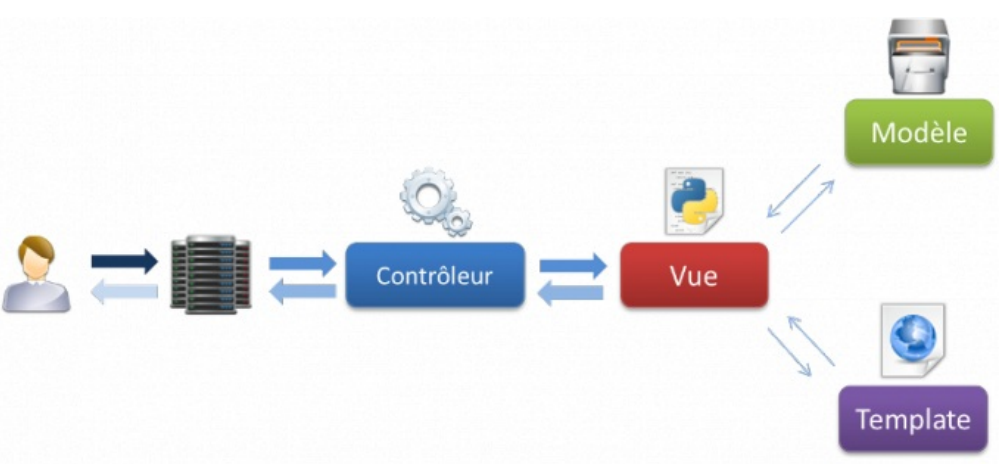
\includegraphics[width=11cm,height=5cm]{images/mvt.png}
\end{column}
\end{columns}
\end{frame}

\subsection{Soaplib}
\begin{frame}
\frametitle{Soaplib}
\framesubtitle{Définition}
\transwipe[duration=2]
\begin{columns}
\begin{column}{8.5cm}
\begin{block}{Définition}<1->
\vspace*{0.1cm}
\begin{itemize}
\item[•] \textcolor{deepgreen}{Soaplib} est une bibliothèque Python facile à utiliser pour la publication des services Web \textcolor{deepred}{SOAP} utilisant \textcolor{deepred}{WSDL 1.1} standard, et la réponse aux demandes \textcolor{deepred}{SOAP 1.1}. 
\item[•] Avec un peu de code, \textcolor{deepgreen}{Soaplib} permet d'écrire un service Web utile et le déployer comme une application \textcolor{deepblue}{WSGI}.
\vspace*{0.3cm}
\end{itemize}
\end{block}
\end{column}
\begin{column}{8.5cm}
\begin{block}{soaplib 2.0.0-beta2}<2->
\vspace*{0.2cm}
\begin{itemize}
\item[•] Publié le 2011-03-15.
\item[•] Disponible à télécharger dans :\\
\textcolor{urlcolor}{\url{https://pypi.python.org/pypi/soaplib/2.0.0-beta2}}\\
\item[•] Documentation officielle:\\
\textcolor{urlcolor}{\url{http://soaplib.github.io/soaplib/2_0/}}
\end{itemize}
\vspace*{0.3cm}
\end{block}
\end{column}
\end{columns}
\end{frame}

\subsection{Java Client Web Service}
\begin{frame}
\frametitle{Java Client Web Service}
\framesubtitle{JAX-WS }
\transwipe[duration=2]
\begin{columns}
\begin{column}{8cm}
\begin{block}{Définition}<1->
\begin{itemize}
\item[•] \textcolor{deepblue}{JAX-WS} (\textcolor{colname}{Java} API for \textcolor{colname}{XML} Web Services) est une API \textcolor{colname}{Java} pour la création des web services.
\item[•] \textcolor{deepblue}{JAX-WS} est l'une des APIs de la programmation \textcolor{colname}{Java/XML}.
\item[•] Elle fait partie du platform \textcolor{colname}{JEE} de SUN Microsystems.
\end{itemize}
\end{block}
\end{column}
\begin{column}{8cm}
\begin{block}{JAX-WS 2.2.10}<2->
\vspace*{0.1cm}
\begin{itemize}
\item[•] Publié le 2015-01-14.\\
\item[•] Disponible à télécharger dans :\\
\textcolor{urlcolor}{\url{https://jax-ws.java.net/2.2.10/}}\\
\item[•] Documentation officielle:\\
\textcolor{urlcolor}{\url{https://jax-ws.java.net/nonav/2.2.10/docs/index.html}}
\end{itemize}
\vspace*{0.2cm}
\end{block}
\end{column}
\end{columns}

\end{frame}
\section{Implémentation}
\subsection{Coté fournisseur}
\begin{frame}
\frametitle{Coté fournisseur (Python)}
\framesubtitle{modèles BDD (models.py)}
%\transblindsvertical[duration=1]
\transsplitverticalout[duration=1.5]
Un modèle est la source d'information unique et définitive à propos de vos données. Il contient les champs et le comportement essentiels des données que vous stockez. Généralement, chaque modèle correspond à une seule table de base de données.
\end{frame}

\begin{frame}
\frametitle{Coté fournisseur (Python)}
\framesubtitle{modèles BDD (MCD)}
%\transblindsvertical[duration=1]
\transsplitverticalout[duration=1.5]
\begin{columns}
\begin{column}{13cm}
\begin{alertblock}{Modèle conceptuel de la BDD}
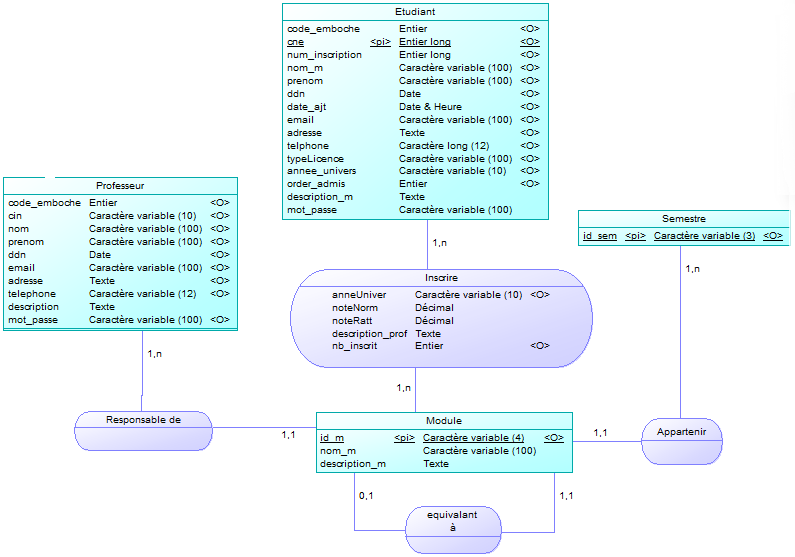
\includegraphics[width=13cm, height=7cm]{images/clientCaptures/mcd.png}
\end{alertblock}
\end{column}
\end{columns}
\end{frame}

\begin{frame}
\frametitle{Coté fournisseur (Python)}
\framesubtitle{modèles Soap (wsmodels.py)}
%\transblindsvertical[duration=1]
\transsplitverticalout[duration=1.5]
Dans \textcolor{deepgreen}{Soaplib}, les types sont les composants responsables de la conversion des paramètres individuels depuis et vers \textcolor{deepblue}{XML}, ainsi que la fourniture des informations nécessaires pour construire le \textcolor{deepblue}{WSDL}. \textcolor{deepgreen}{Soaplib} a beaucoup de types intégrés qui vous donnent la plupart des types de données communs généralement nécessaires.
\end{frame}


\begin{frame}
\frametitle{Coté fournisseur (Python)}
\framesubtitle{Service Etudiant (views.py)}
%\transblindsvertical[duration=1]
\transsplitverticalout[duration=1.5]
Ce fichier contient généralement les différents services. Dans notre cas il ne contient qu'un seul service \textcolor{backgroundcolor}{\textbf{EtudiantService}} et ses méthodes que le client va les appeler.
\end{frame}

\subsection{Coté Consommateur}
\begin{frame}
\frametitle{Coté Consommateur (Java)}
\framesubtitle{Créer projet (Netbeans)}
%\transblindsvertical[duration=1]
\transboxin[duration=1]
\begin{columns}
\begin{column}{16cm}
 \begin{alertblock}{Créer nouveau projet}
 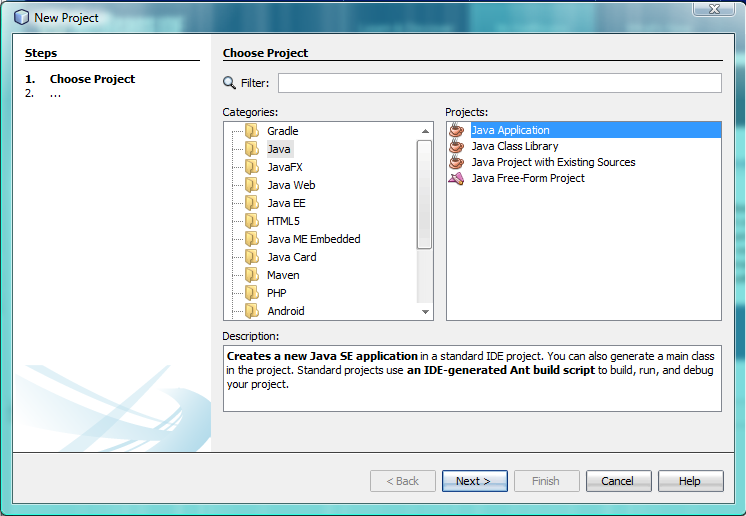
\includegraphics[width=16cm,height=7.2cm]{images/clientCaptures/etape1_new_project.png}
  \end{alertblock}
\end{column}
\end{columns}
\end{frame}

\begin{frame}
\frametitle{Coté Consommateur (Java)}
\framesubtitle{Créer projet (Netbeans)}
%\transblindsvertical[duration=1]
\transsplithorizontalin[duration=1]
\begin{columns}
\begin{column}{16cm}
 \begin{alertblock}{Créer nouveau projet}
 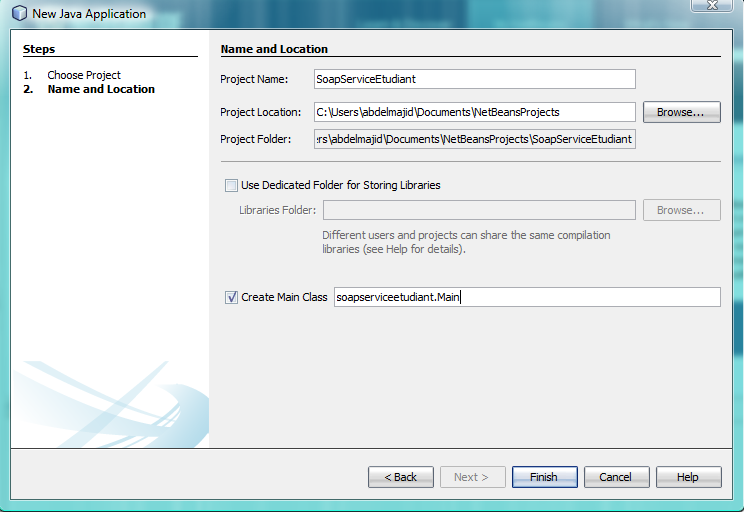
\includegraphics[width=16cm,height=7.2cm]{images/clientCaptures/etape2_new_project.png}
  \end{alertblock}
\end{column}
\end{columns}
\end{frame}


\begin{frame}
\frametitle{Coté Consommateur (Java)}
\framesubtitle{Importer au sein du projet un web service (Netbeans)}
%\transblindsvertical[duration=1]
\transsplithorizontalin[duration=1]
\begin{columns}
\begin{column}{16cm}
 \begin{alertblock}{Créer un Web Service Client}
 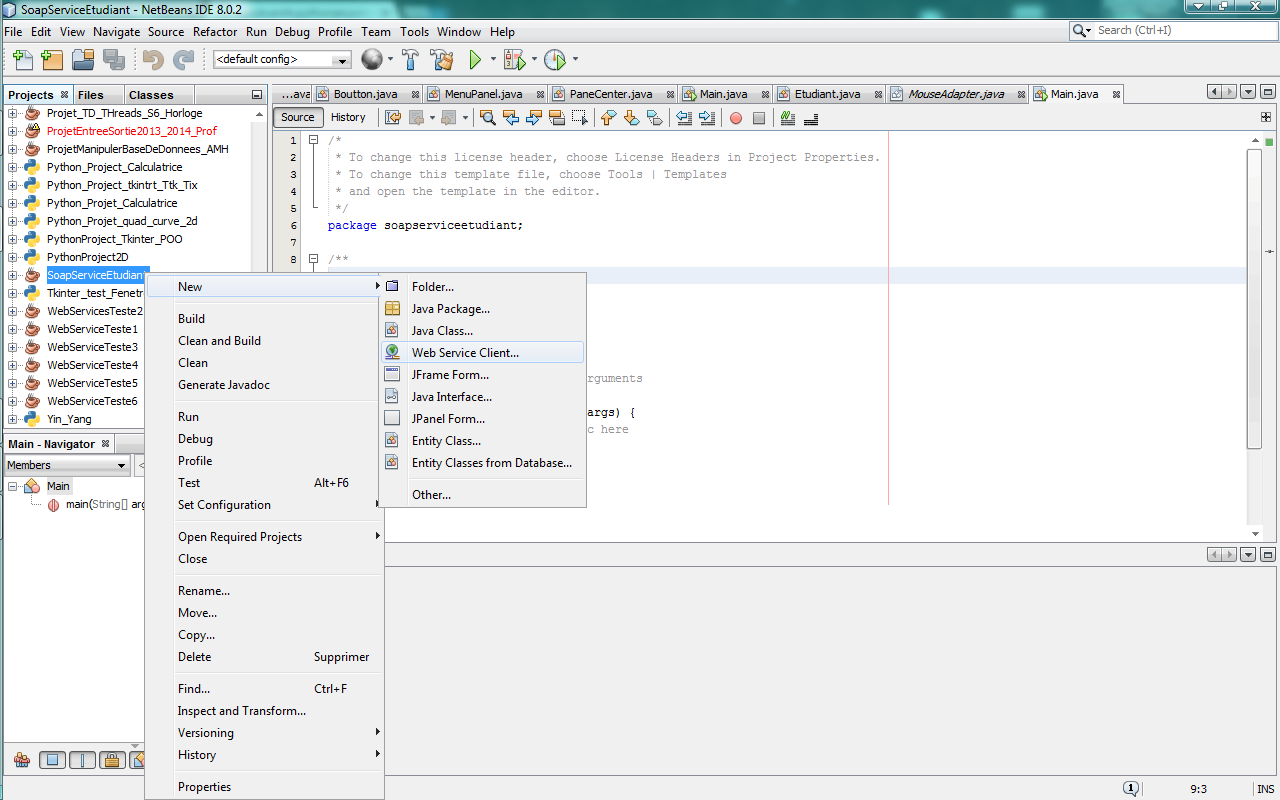
\includegraphics[width=16cm,height=7.2cm]{images/clientCaptures/etape3_client_web_service.png}
  \end{alertblock}
\end{column}
\end{columns}
\end{frame}

\begin{frame}
\frametitle{Coté Consommateur (Java)}
\framesubtitle{Préciser l'url du ficher WSDL (Netbeans)}
%\transblindsvertical[duration=1]
\transsplithorizontalin[duration=1]
\begin{columns}
\begin{column}{16cm}
 \begin{alertblock}{Url du fichier WSDL}
 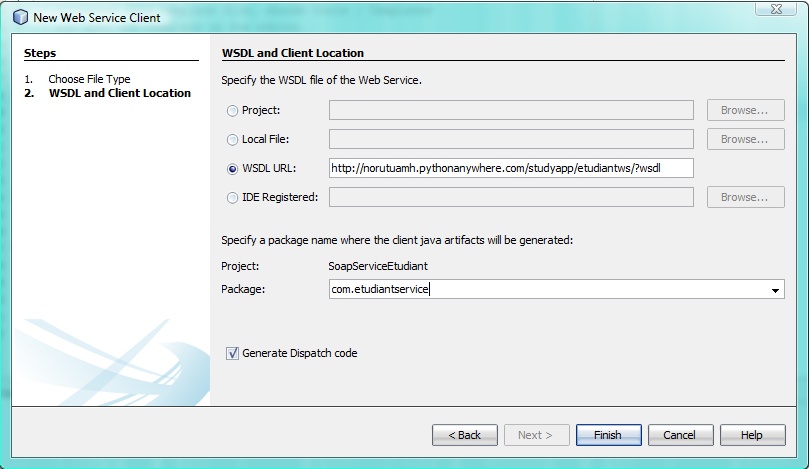
\includegraphics[width=16cm,height=7.2cm]{images/clientCaptures/etape5_client_web_service_wsdl.png}
  \end{alertblock}
\end{column}
\end{columns}
\end{frame}

\begin{frame}
\frametitle{Coté Consommateur (Java)}
\framesubtitle{Composantes importées (Netbeans)}
%\transblindsvertical[duration=1]
\transsplithorizontalin[duration=1]
\begin{columns}
\begin{column}{10cm}
 \begin{alertblock}{}
 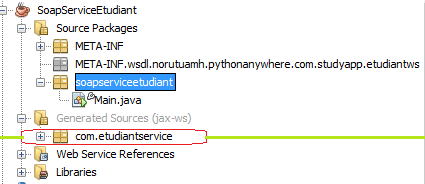
\includegraphics[width=10cm,height=5cm]{images/clientCaptures/etape6_projet_genere.png}
  \end{alertblock}
\end{column}
\end{columns}
\end{frame}

\begin{frame}
\frametitle{Coté Consommateur (Java)}
\framesubtitle{Package contenant les différents types et fonctions du WS (Netbeans)}
%\transblindsvertical[duration=1]
\transsplithorizontalin[duration=1]
\begin{columns}
\begin{column}{8cm}
 \begin{alertblock}{}
 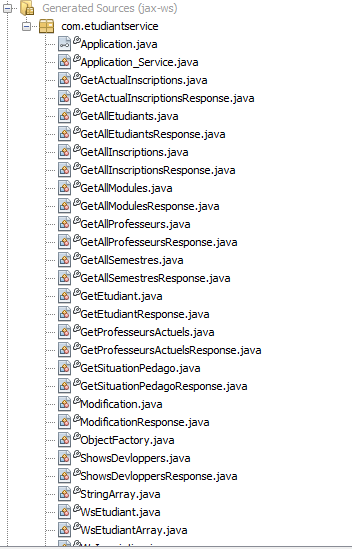
\includegraphics[width=8cm,height=8cm]{images/clientCaptures/etape7_package_fonctions_responses_types.png}
  \end{alertblock}
\end{column}
\end{columns}
\end{frame}

\begin{frame}
\frametitle{Coté Consommateur (Java)}
\framesubtitle{Contenu d'application de web service (Netbeans)}
%\transblindsvertical[duration=1]
\transsplithorizontalin[duration=1]
\begin{columns}
\begin{column}{14cm}
 \begin{alertblock}{Les opérations ou bien les fonctions du WS}
 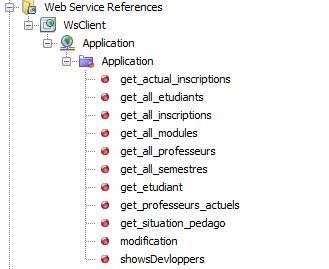
\includegraphics[width=14cm,height=7cm]{images/clientCaptures/etape8_servives_utilisess.png}
  \end{alertblock}
\end{column}
\end{columns}
\end{frame}

\begin{frame}
\frametitle{Coté Consommateur (Java)}
\framesubtitle{Compléter le projet Java (Netbeans)}
%\transblindsvertical[duration=1]
\transsplithorizontalin[duration=1]
\begin{columns}
\begin{column}{16cm}
 \begin{alertblock}{Importer une fonction dans notre projet Java.}
 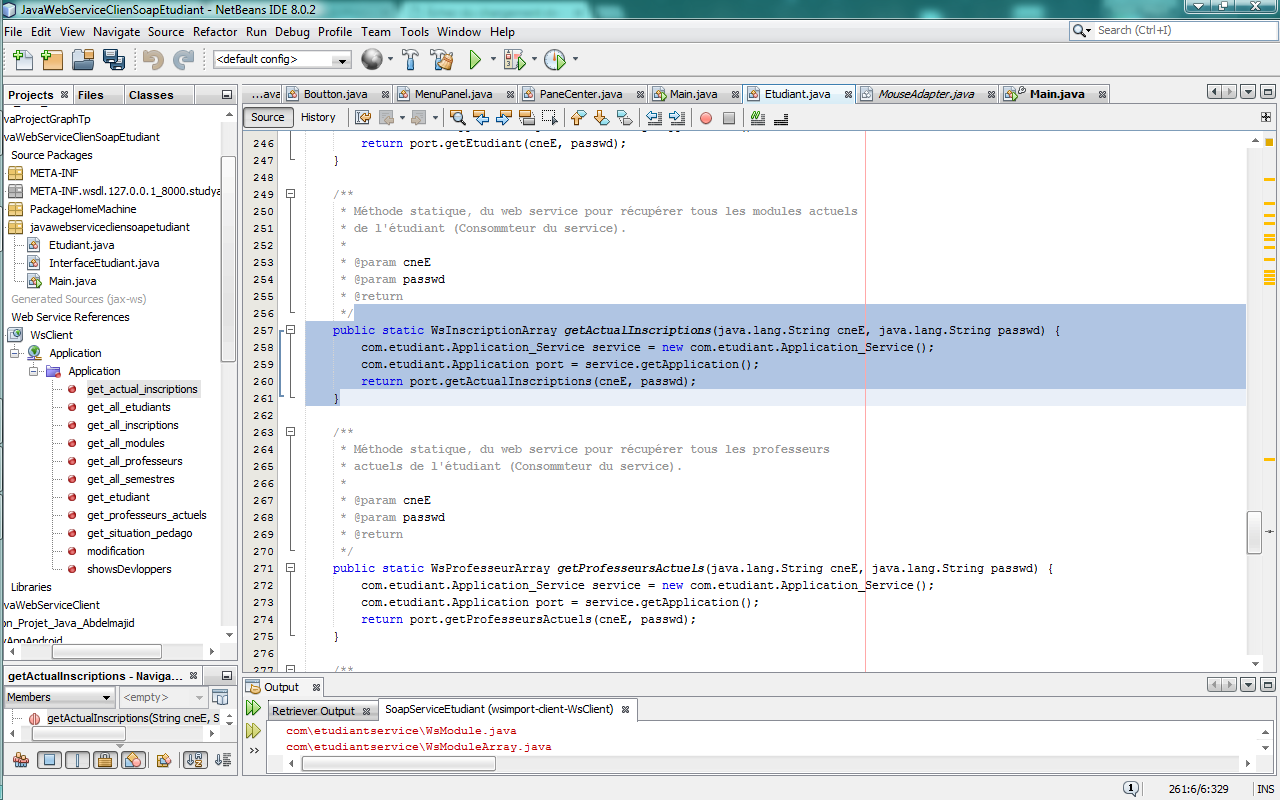
\includegraphics[width=16cm,height=7.2cm]{images/clientCaptures/etape9_importer_procedure.png}
  \end{alertblock}
\end{column}
\end{columns}
\end{frame}


\section{Démonstration}

\begin{frame}
\transglitter[duration=2]
\frametitle{Démonstration}
%\framesubtitle{Web}

\begin{columns}
\begin{column}{9cm}
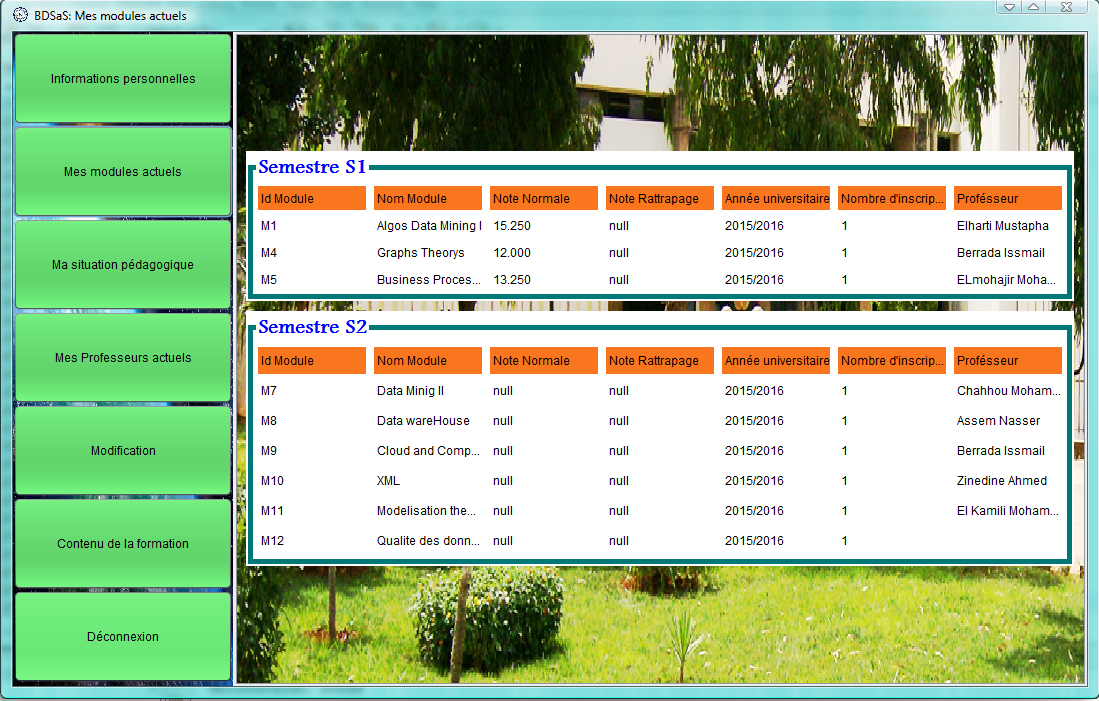
\includegraphics[width=0.5\paperwidth,height=0.5\paperheight]{images/etd_service.png}
\end{column}

\begin{column}{9cm}
\begin{center}
\begin{Huge}
\textbf{
\color{cell2}
\color{deepblue}
Démonstration ... 
\begin{flushright}
\color{backgroundcolor}
\begin{normalsize}
\textit{EtudiantService}
\end{normalsize}
\end{flushright}
}
\end{Huge}
\end{center}
\end{column}
\end{columns}

\end{frame}

%\input{sections/implementationPython}
%\input{sections/distributionsPython}
%\input{sections/frameworkspython}
%\input{sections/pythonscientifique}
	%\input{sections/progsystemPython}
	%\input{sections/devmobilpython}
	%\input{sections/pythonsecurity}
	%\input{sections/networkpython}
%\input{sections/bigdataPython}
%\input{sections/pratiquepython}
\section{Conclusion}

\usebackgroundtemplate{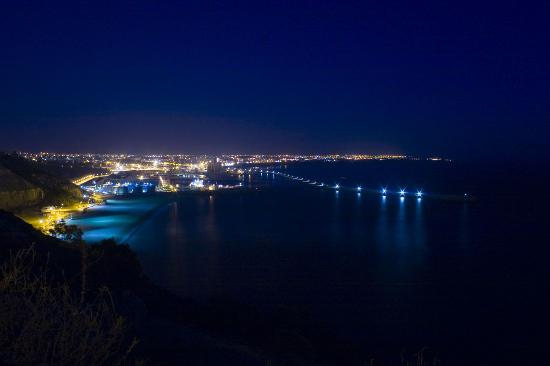
\includegraphics[width=\paperwidth,height=\paperheight]{images/safi.jpg}}
\begin{frame}[plain]
\transglitter[duration=2.5]
%\includegraphics[width=0.95\textwidth]{imgs/merci.png}

\begin{center}
\begin{Huge}

\textbf{
\color{white}
Merci... \\[5cm]
\begin{flushright}
\color{yellow}
<Questions/> \\
et\\
<Réponses/>
\end{flushright}
%\begin{flushright}
%\color{purple}
%\textit{Albert Einstein}
%\end{flushright}
}

\end{Huge}
\end{center}
\end{frame}

%(EXPOSION) éclaircissage des données des groupes par integration des graphes
%\setbeamertemplate{background}[default]%aucien fond
%
%\begin{frame}[label=labele]
%\frametitle{Introduction}
%c'est l'introduction \textcolor{titre}{titre}
%\begin{itemize}
%\item Python
%\item automates
%\item PADA
%\end{itemize}
%\end{frame}
%\begin{frame}[fragile]
%\hyperlinkmovie[showcontrols]{videos/vid.mp4}{videos/vid.mp4}
%\movie[autostart]{}{videos/vid.mp4}
%\url{videos/vid.mp4}
%toto titi
%\end{frame}
%\begin{frame}
%\frametitle{BLOCK}
%\begin{block}{Bloc standard}
%Un bloc tout simple,
%par défaut un texte
%sur un fond de couleur
%qui dépend, bien sûr,
%du thème choisi.
%\end{block}
%\end{frame}
%\begin{frame}
%\frametitle{BLOCK}
%\begin{block}{Un bloc normal}
%Texte du block \texttt{block}
%\end{block}
%\begin{alertblock}{Un bloc très alerte}
%Texte du block \texttt{alertblock}
%\end{alertblock}
%\begin{exampleblock}{Un bloc exemplaire}
%Exemple de block \texttt{exampleblock}
%\end{exampleblock}
%\end{frame}
%\begin{frame}
%\frametitle{colonnes}
%\begin{columns}
%\begin{column}{6cm}
%Contenu de ma première colonne
%\end{column}
%\begin{column}{6cm}
%Contenu de ma deuxième colonne
%\end{column}
%\end{columns}
%\end{frame}
%\begin{frame}
%\frametitle{animations}
%Voici ma première idée, je cause, je cause...
%\pause Voici la deuxième idée que j'affiche quand je suis prête à en causer.
%\pause Voici la troisième idée après réflexion.
%\end{frame}
%\begin{frame}
%\frametitle{animations}
%\begin{itemize}
%\item<3-> l'élément de liste apparaîtra depuis
%la couche numéro 3.
%\item<2-> l'élément de liste apparaîtra
%en gras sur la couche 2 puis normalement.
%\item<1-> \textbf<2>{l'élément de liste apparaîtra} depuis
%la couche numéro 1.
%\end{itemize}
%\end{frame}

\end{document}